% CaelumFusion VGA Rendering Configuration and Control Map - Phase 6
% Source-aligned engineering draft for the Basys-3 VGA rendering path.
%
% This document intentionally contains no HDMI/TMDS output contract.  The
% project target described here is the Digilent Basys-3 VGA output path only.
% The package set is kept intentionally conservative so it compiles with the
% bundled offline Tectonic cache used in this Codex environment.

\documentclass{article}

\usepackage[margin=0.75in]{geometry}
\usepackage{amsmath}
\usepackage{amssymb}
\usepackage{array}
\usepackage{booktabs}
\usepackage{longtable}
\usepackage{tabularx}
\usepackage{enumitem}
\usepackage{xcolor}
\usepackage{graphicx}
\usepackage{tikz}
\usetikzlibrary{arrows.meta}
\usepackage{listings}
\usepackage[hidelinks]{hyperref}

\setlength{\parindent}{0pt}
\setlength{\parskip}{5pt}
\renewcommand{\arraystretch}{1.18}
\setlist[itemize]{leftmargin=1.4em,itemsep=2pt,topsep=3pt}
\setlist[enumerate]{leftmargin=1.6em,itemsep=2pt,topsep=3pt}

\lstset{
  basicstyle=\normalsize,
  breaklines=true,
  columns=fullflexible,
  keepspaces=true,
  frame=single,
  framerule=0.2pt,
  xleftmargin=0.4em,
  xrightmargin=0.4em
}

\urlstyle{same}
\newcommand{\docname}{CaelumFusion\_VGA\_Rendering\_Configuration\_and\_Control\_Map\_Phase\_6}
\newcommand{\sig}[1]{\begingroup\nolinkurl{#1}\endgroup}
\newcommand{\file}[1]{\begingroup\nolinkurl{#1}\endgroup}
\newcommand{\param}[1]{\begingroup\nolinkurl{#1}\endgroup}
\newcommand{\yes}{\textsc{yes}}
\newcommand{\no}{\textsc{no}}
\newcommand{\na}{\textsc{n/a}}

\title{\textbf{CaelumFusion VGA Rendering Configuration and Control Map}\\Phase 6}
\author{CaelumFusion Flight Control Project}
\date{Draft generated July 5, 2026}

\begin{document}
\maketitle

\begin{center}
\fbox{\begin{minipage}{0.92\linewidth}
\textbf{Scope correction.}  This document is a fresh VGA-only engineering
draft for the CaelumFusion Basys-3 rendering path.  The project described here
does not use HDMI, TMDS, DisplayPort, or a digital video encoder.  The only
board-facing display interface in scope is the Basys-3 analog VGA connector,
driven by \sig{vga_hsync}, \sig{vga_vsync}, and \sig{vga_rgb[11:0]}.
\end{minipage}}
\end{center}

\tableofcontents
\listoffigures
\listoftables
\newpage

\section{Purpose}

The purpose of \docname{} is to define the Phase 6 VGA rendering configuration
and control map for the CaelumFusion flight-control visualization system.  The
document is written as an engineering control artifact rather than a marketing
description: every visible screen element, control input, timing assumption, and
clock-domain boundary is tied back to the current RTL or to a clearly marked
Phase 6 integration target.

The immediate goals are:
\begin{itemize}
  \item remove the earlier HDMI misunderstanding from the project narrative;
  \item document the actual Basys-3 VGA output contract;
  \item distinguish the implemented top-level path from the Phase 6 render
        unification wrapper now present in the source tree;
  \item preserve the semantic distinction between raw telemetry, derived state,
        diagnostic page output, self-test stimulus, and final VGA pixels;
  \item provide a verification checklist suitable for RTL review, simulation,
        implementation signoff, and bench bring-up.
\end{itemize}

\section{Scope and Non-Scope}

\subsection{In Scope}

\begin{itemize}
  \item Digilent Basys-3 / Artix-7 board-facing VGA output.
  \item 640 by 480 active-video timing generated from a 25.000 MHz pixel clock.
  \item 12-bit RGB output in the form \sig{\{R[3:0], G[3:0], B[3:0]\}}.
  \item SYS-domain telemetry normalization into the packed visualization bundle.
  \item SYS-to-PIX snapshot CDC and frame-boundary visual commit.
  \item Flight HUD rendering, text overlay, history charts, attitude/heading
        instruments, apogee authority visualization, landing/wind viewport, and
        bottom engineering strip.
  \item Optional full-screen planar compass truth page overlay.
  \item Phase 6 render-view control states for normal HUD, compass truth page,
        and self-test HUD stimulus.
\end{itemize}

\subsection{Explicitly Out of Scope}

\begin{itemize}
  \item HDMI, TMDS, DVI, DisplayPort, MIPI, or any digital-video encoder.
  \item HDMI pixel repetition, data-enable generation, TMDS clocking, or 8b/10b
        style video serialization.
  \item EDID, monitor negotiation, audio, HDCP, or hot-plug detection.
  \item Any claim that the Basys-3 VGA pins are an HDMI bridge.  They are not.
\end{itemize}

\section{Authoritative Source Inputs}

This draft is grounded in the current Vivado checkout rather than in the
previous HDMI-oriented document.  The legacy report is treated as historical
context; the implementation contracts below are taken from the active RTL,
constraints, and verification artifacts in this checkout.

\begin{longtable}{p{0.34\linewidth} p{0.58\linewidth}}
\toprule
\textbf{Source file} & \textbf{Contract used in this document} \\
\midrule
\endhead
\file{CaelumFusion_Flight_Control_System.srcs/sources_1/new/caelumfusion_top_vga.v} &
Canonical board-facing integration top.  Owns the 100 MHz board clock input,
pixel clock generation, sensor publication layer, authority gate producer,
board-control synchronization/debounce, render-control wrapper instantiation,
and final VGA ports. \\

\file{CaelumFusion_Flight_Control_System.srcs/sources_1/new/caelumfusion_vga_render_control.v} &
Phase 6 render-control unification wrapper.  Defines legal render views,
direct/next/previous selection, invalid-view latch, and split self-test versus
compass-page enable semantics.  This is the active VGA compositor boundary
inside \file{caelumfusion_top_vga.v}. \\

\file{CaelumFusion_Flight_Control_System.srcs/sources_1/new/flight_viz_suite_top.v} &
End-to-end flight visualization shell.  Selects self-test or live telemetry,
normalizes SYS-domain evidence into a canonical visualization bundle, transfers
the bundle to PIX, stores history rings, and instantiates the PIX renderer. \\

\file{CaelumFusion_Flight_Control_System.srcs/sources_1/new/flight_viz_model_sys.v} &
SYS-domain semantic packing layer.  Converts sensor summaries, derived state,
authority evidence, navigation and wind fields, power evidence, and metadata
into the canonical visualization bundle. \\

\file{CaelumFusion_Flight_Control_System.srcs/sources_1/new/flight_visualizer_pix.v} &
PIX-domain VGA renderer.  Generates 640 by 480 timing, commits semantic updates
at frame boundaries, renders base instruments, composites text, and drives final
\sig{vga_hsync}, \sig{vga_vsync}, and \sig{vga_rgb}. \\

\file{CaelumFusion_Flight_Control_System.srcs/sources_1/new/flight_viz_telemetry_textgen.v} &
PIX-domain text source.  Converts committed telemetry fields into fixed-width
ASCII line buses and assigns semantic RGB colors for raw, derived, and bottom
debug text. \\

\file{CaelumFusion_Flight_Control_System.srcs/sources_1/new/flight_viz_telemetry_compositor.v} &
PIX-domain text placement and glyph compositor.  Defines fixed origins, clip
bands, glyph scale, and priority order for top, panel, and bottom text. \\

\file{CaelumFusion_Flight_Control_System.srcs/sources_1/new/flight_vga_page_mux_pix.v} &
PIX-domain final page selector inside the normal HUD renderer.  Selects between
the primary HUD scene and the optional sensor-diagnostic page, applies active
video blacking, and prevents normal telemetry text from occluding the diagnostic
page. \\

\file{CaelumFusion_Flight_Control_System.srcs/sources_1/new/planar_compass_truth_page_vga.v} &
Optional full-screen diagnostic overlay.  Passes the existing VGA stream through
when inactive and replaces RGB with the compass truth page when active. \\

\file{CaelumFusion_Flight_Control_System.srcs/sources_1/new/vga_timing_640x480_60.v} &
Registered VGA timing generator with active-video, coordinate, sync, and
\sig{vsync_edge} outputs. \\

\file{CaelumFusion_Flight_Control_System.srcs/sources_1/new/flight_viz_bundle_defs.vh} &
Canonical 1152-bit visualization bundle field map. \\

\file{CaelumFusion_Flight_Control_System.srcs/sources_1/new/flight_viz_bundle_cdc.v} &
Low-rate snapshot CDC from SYS to PIX using a stable source hold register and a
synchronized toggle event. \\

\file{CaelumFusion_Flight_Control_System.srcs/constrs_1/new/Basys-3-Master.xdc} &
Basys-3 pin mapping, 100 MHz input clock constraint, VGA pin assignments, and
scoped SYS-to-PIX CDC false paths. \\

\file{CaelumFusion_Flight_Control_System.srcs/sim_1/new/tb_flight_visualizer_pix.v} &
PIX renderer proof checks for overlay priority, color packing, clipping,
inactive-video blacking, charts, attitude instruments, apogee ladder, and debug
strip. \\

\file{CaelumFusion_Flight_Control_System.srcs/sim_1/new/tb_flight_viz_suite_top.v} &
Suite-level transport-and-render proof for SYS publication, CDC delivery,
history-ring capture, and visible VGA pixel response. \\

\file{docs/CaelumFusion_L1_Avionics_Release_Checklist.md} &
Release-gate expectations for Basys-3 \file{caelumfusion_top_vga}, including
simulation, timing, DRC, hardware bench, and VGA/HUD evidence. \\
\bottomrule
\end{longtable}

\section{Board-Facing VGA Contract}

\subsection{Physical Display Interface}

The display path terminates at the Basys-3 VGA connector.  The FPGA drives
horizontal sync, vertical sync, and 12 one-bit GPIO-style color outputs through
the board's resistor DAC network.  The color bus is logically packed as:

\begin{center}
\sig{vga_rgb[11:0]} = \sig{\{red[3:0], green[3:0], blue[3:0]\}}
\end{center}

The XDC maps the individual color bits as follows.

\begin{center}
\begin{tabular}{c c c c}
\toprule
\textbf{Color} & \textbf{Logical bits} & \textbf{Package pins} & \textbf{I/O standard} \\
\midrule
Red   & \sig{vga_rgb[11:8]} & \sig{G19,H19,J19,N19} & LVCMOS33 \\
Green & \sig{vga_rgb[7:4]}  & \sig{J17,H17,G17,D17} & LVCMOS33 \\
Blue  & \sig{vga_rgb[3:0]}  & \sig{N18,L18,K18,J18} & LVCMOS33 \\
\bottomrule
\end{tabular}
\end{center}

Sync outputs are:
\begin{center}
\begin{tabular}{c c c}
\toprule
\textbf{Signal} & \textbf{Package pin} & \textbf{Default polarity} \\
\midrule
\sig{vga_hsync} & \sig{P19} & active low, \param{HSYNC_POL=0} \\
\sig{vga_vsync} & \sig{R19} & active low, \param{VSYNC_POL=0} \\
\bottomrule
\end{tabular}
\end{center}

\subsection{Board Switch and Button Mapping}

The top-level board controls are not all display-mode controls.  Two switches
feed the apogee authority gate and therefore change rendered authority evidence;
the remaining configured buttons and switches are synchronized before reaching
the render-control wrapper or runtime sensor-control gates.  The mapping below
is from the checked XDC and \file{caelumfusion_top_vga.v}.

\begin{longtable}{p{0.16\linewidth} p{0.19\linewidth} p{0.20\linewidth} p{0.36\linewidth}}
\toprule
\textbf{Board item} & \textbf{RTL signal} & \textbf{Package pin} & \textbf{Rendering effect} \\
\midrule
\endhead
100 MHz oscillator &
\sig{clk} &
\sig{W5} &
Feeds SYS logic and the MMCM that generates the 25 MHz pixel clock. \\

Reset button &
\sig{rst} &
\sig{U18} &
Resets SYS integration and pixel-domain rendering state.  VGA output returns to
deterministic idle/black until timing and committed telemetry resume. \\

SW0 &
\sig{sw_arm_raw} &
\sig{V17} &
Software-arm input to the authority gate.  It changes the apogee authority gate
strip, command permissive color, and related policy evidence; it is not a view
selector. \\

SW1 &
\sig{sw_policy_enable_raw} &
\sig{V16} &
Runtime policy-enable input to the authority gate.  It changes the authority
policy/gate display state; it is not a VGA page selector. \\

BTNU &
\sig{btn_page_raw} &
\sig{T18} &
Debounced one-cycle \sig{view_next_pulse_sys}.  Cycles the registered view
selection in \file{caelumfusion_vga_render_control.v}. \\

BTND &
\sig{btn_prev_raw} &
\sig{U17} &
Debounced one-cycle \sig{view_prev_pulse_sys}.  Cycles the registered view
selection in reverse order. \\

BTNR &
\sig{btn_direct_compass_raw} &
\sig{T17} &
Debounced direct-view request.  In the active encoded-selector RTL, BTNR loads
SW13:SW11 only while SW3 MAG1 bench mode and SW2+SW6 diagnostic fault injection
are inactive; during either ownership mode the request is forced to reserved
\sig{3'b111} and rejected.  With encoded selection disabled, BTNR requests
\sig{VIEW_COMPASS_TRUTH}. \\

SW2 &
\sig{sw_selftest_raw} &
\sig{W16} &
Level-style \sig{legacy_selftest_hold_sys}; selects the self-test HUD unless a
compass-page hold has priority. \\

SW3 &
\sig{sw_mag1_bench_raw} &
\sig{W17} &
Enables the synthetic MAG1 bench source when the corresponding build parameter
allows it. \\

SW4 &
\sig{sw_compass_page_raw} &
\sig{W15} &
Level-style \sig{legacy_compass_page_hold_sys}; forces
\sig{VIEW_COMPASS_TRUTH} when the page is present. \\

SW5 &
\sig{sw_history_freeze_raw} &
\sig{V15} &
Freezes PIX-domain HUD history updates through \sig{history_freeze_sys}. \\

SW6 &
\sig{sw_log_diag_raw} &
\sig{W14} &
Runtime enable for black-box/log diagnostic emission; with SW2 high it enables
deliberate diagnostic fault injection. \\

SW7--SW10 &
\sig{sw_lis3dh_i2c_acc_raw}, \sig{sw_adxl362_spi_acc_raw},
\sig{sw_cmps2_mmc3416_mag_raw}, \sig{sw_pmon1_pwr_raw} &
\sig{W13}, \sig{V2}, \sig{T3}, \sig{T2} &
Runtime sensor-path enables gated by the corresponding compile-time
\param{USE_*} parameters. \\

SW11--SW13 &
\sig{sw_mag1_offset_x_raw}, \sig{sw_mag1_offset_y_raw},
\sig{sw_mag1_offset_z_raw} &
\sig{R3}, \sig{W2}, \sig{U1} &
Applies MAG1 bench-source offset controls for redundant-magnetometer testing.
With SW2+SW6 they select diagnostic fault class.  Otherwise, in encoded-selector
builds, they provide the BTNR direct-view ID bits. \\

SW14 &
\sig{sw_compass_default_raw} &
\sig{T1} &
Runtime companion hold for the compass/MAG evidence page.  It is ORed with SW4
at the top-level render-control boundary. \\

SW15 &
\sig{sw_ext_i2c_raw} &
\sig{R2} &
Runtime enable for the optional shared-I2C extension group; extension evidence
degrades unavailable when the compiled or runtime gate is low. \\
\bottomrule
\end{longtable}

\begin{center}
\begin{tabularx}{\linewidth}{p{0.24\linewidth} X}
\toprule
\textbf{Control class} & \textbf{Current status} \\
\midrule
Direct view next/previous & Implemented inside
\file{caelumfusion_vga_render_control.v} as \sig{view_next_pulse_sys} and
\sig{view_prev_pulse_sys}, and wired to BTNU/BTND through debounced SYS-domain
pulses. \\
Direct view ID select & Implemented inside the Phase 6 wrapper through
\sig{view_direct_valid_sys} and \sig{view_direct_id_sys}; in the current
encoded-selector RTL, BTNR samples SW13:SW11 only when SW3 and SW2+SW6 fault
injection are inactive.  During those SW11--SW13 ownership modes the request is
forced to reserved \sig{3'b111}. \\
Widget-level enables & Not exposed as top-level board controls.  Most widgets
are always rendered and degrade through validity/freshness/status color or
hatching instead of disappearing. \\
\bottomrule
\end{tabularx}
\end{center}

\subsection{Clock Plan}

The board input clock is the Basys-3 100.000 MHz oscillator on \sig{clk}.  The
clock-generation wrapper converts it to a 25.000 MHz pixel clock with an MMCM:

\[
  F_{\mathrm{VCO}}
  = 100.000\,\mathrm{MHz} \times \frac{10.000}{1}
  = 1000.000\,\mathrm{MHz}
\]

\[
  F_{\mathrm{pix}}
  = \frac{1000.000\,\mathrm{MHz}}{40.000}
  = 25.000\,\mathrm{MHz}.
\]

The 25.000 MHz pixel clock is a practical Basys-3 lab-compatible approximation
to the nominal 25.175 MHz VGA pixel clock.  With the configured 800 by 525
total raster, the realized frame rate is:

\[
  F_{\mathrm{frame}}
  = \frac{25.000\,\mathrm{MHz}}{800 \times 525}
  \approx 59.524\,\mathrm{Hz}.
\]

\subsection{VGA Timing Parameters}

\begin{center}
\begin{tabular}{l r r l}
\toprule
\textbf{Dimension} & \textbf{Parameter} & \textbf{Value} & \textbf{Meaning} \\
\midrule
Horizontal active & \param{H_ACTIVE} & 640 & visible pixels \\
Horizontal front porch & \param{H_FP} & 16 & post-active blanking \\
Horizontal sync & \param{H_SYNC} & 96 & sync pulse width \\
Horizontal back porch & \param{H_BP} & 48 & pre-active blanking \\
Horizontal total & derived & 800 & complete line clocks \\
\midrule
Vertical active & \param{V_ACTIVE} & 480 & visible lines \\
Vertical front porch & \param{V_FP} & 10 & post-active blanking \\
Vertical sync & \param{V_SYNC} & 2 & sync pulse height \\
Vertical back porch & \param{V_BP} & 33 & pre-active blanking \\
Vertical total & derived & 525 & complete frame lines \\
\bottomrule
\end{tabular}
\end{center}

\section{Implemented Rendering Architecture}

\subsection{Current Board Path}

Figure~\ref{fig:implemented-path} shows the currently implemented
\file{caelumfusion_top_vga.v} display path.  The important engineering point is
that the final output is a VGA stream at all times.  When the optional compass
truth page is not synthesized or not active, \sig{vga_rgb} is simply the normal
flight HUD output.  When the optional page is synthesized and active, only RGB
is replaced by the diagnostic page; sync is passed through.

\begin{figure}[h]
\centering
\resizebox{\linewidth}{!}{%
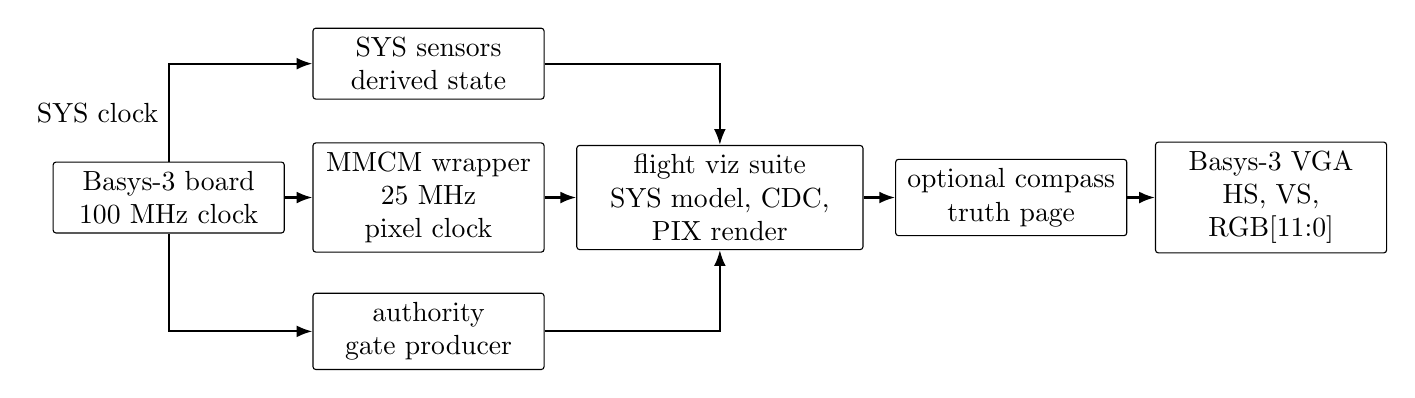
\begin{tikzpicture}[
  box/.style={draw, rounded corners=1pt, text width=2.7cm, minimum height=0.9cm, align=center},
  wide/.style={draw, rounded corners=1pt, text width=3.4cm, minimum height=1.0cm, align=center},
  arr/.style={-{Latex[length=2mm]}, thick}
]
\node[box]  at (0,0)    (clk)     {Basys-3 board\\100 MHz clock};
\node[box]  at (3.3,0)  (mmcm)    {MMCM wrapper\\25 MHz pixel clock};
\node[wide] at (7.0,0)  (suite)   {flight viz suite\\SYS model, CDC, PIX render};
\node[box]  at (10.7,0) (truth)   {optional compass\\truth page};
\node[box]  at (14.0,0) (pins)    {Basys-3 VGA\\HS, VS, RGB[11:0]};
\node[box]  at (3.3,1.7) (sensors){SYS sensors\\derived state};
\node[box]  at (3.3,-1.7) (auth)  {authority\\gate producer};

\draw[arr] (clk) -- (mmcm);
\draw[arr] (mmcm) -- (suite);
\draw[arr] (suite) -- (truth);
\draw[arr] (truth) -- (pins);
\draw[arr] (sensors) -| (suite);
\draw[arr] (auth) -| (suite);
\draw[arr] (clk) |- node[pos=0.25,left]{SYS clock} (sensors);
\draw[arr] (clk) |- (auth);
\end{tikzpicture}}
\caption{Implemented board-facing VGA rendering path.}
\label{fig:implemented-path}
\end{figure}

\subsection{Module Responsibilities}

\begin{longtable}{p{0.28\linewidth} p{0.63\linewidth}}
\toprule
\textbf{Module} & \textbf{Rendering responsibility} \\
\midrule
\endhead
\file{caelumfusion_top_vga} &
Board integration.  Selects I2C/SPI sensor suite variant, generates pixel clock
and reset, routes sensor and derived evidence into visualization, connects
\sig{btn_page_raw}, and exposes final VGA pins. \\

\file{flight_viz_suite_top} &
System-level visualization shell.  Provides self-test substitution, normalizes
raw and derived telemetry into the 1152-bit visualization bundle, publishes
semantic changes across CDC, stores altitude and vertical-speed history rings,
and instantiates the pixel renderer. \\

\file{flight_viz_model_sys} &
SYS-domain semantic model.  Converts source summaries, derived state,
navigation/wind context, authority gates, power evidence, and metadata into the
canonical packed bundle. \\

\file{flight_viz_bundle_cdc} &
CDC bridge.  Holds the published bundle stable in SYS and transfers an event to
PIX through a three-stage toggle synchronizer. \\

\file{flight_visualizer_pix} &
PIX-domain visual renderer.  Generates timing, freezes the bundle at
frame-boundary commits, renders base instrumentation, composites text, and
forces RGB black outside active video. \\

\file{flight_viz_telemetry_textgen} &
Converts committed PIX-domain telemetry fields into fixed-width ASCII line buses
and semantic RGB colors. \\

\file{flight_viz_telemetry_compositor} &
Places fixed text objects into top, panel, and bottom bands using a shared
3-by-5 glyph datapath. \\

\file{planar_compass_truth_page_vga} &
Optional full-screen magnetic-heading diagnostic page.  It is additive and
passes the existing VGA stream through unchanged when inactive. \\
\bottomrule
\end{longtable}

\section{Phase 6 Render-Control Boundary}

\subsection{Why the Control Boundary Exists}

The board top now routes visible-display selection through
\file{caelumfusion_vga_render_control.v}.  This boundary keeps three engineering
states separate:

\begin{itemize}
  \item registered view selection from debounced next/previous/direct pulses;
  \item level-style compass-page and self-test holds from synchronized switches;
  \item final VGA compositing between the normal HUD stream and the optional
        full-screen compass/MAG evidence page.
\end{itemize}

This removes the early bring-up coupling where one raw button simultaneously
requested the truth page and substituted deterministic self-test evidence into
the hidden HUD.  A full-screen magnetic truth page is now a visible page
selection, the sensor diagnostics page is a page-selectable HUD-renderer mode,
and self-test remains an explicit HUD stimulus selection.

\subsection{Legal View States}

\begin{center}
\begin{tabularx}{\linewidth}{p{0.13\linewidth} p{0.24\linewidth} X}
\toprule
\textbf{View ID} & \textbf{Name} & \textbf{Visible result} \\
\midrule
\sig{3'd0} & \sig{VIEW_FLIGHT_HUD} &
Normal flight HUD driven by live telemetry and derived estimates. \\
\sig{3'd1} & \sig{VIEW_COMPASS_TRUTH} &
Full-screen planar compass / magnetometer truth page. \\
\sig{3'd2} & \sig{VIEW_SELFTEST_HUD} &
Normal flight HUD driven by deterministic renderer self-test stimulus. \\
\sig{3'd3} & \sig{VIEW_SENSOR_DIAG} &
HUD-renderer diagnostic page for sensor validity, extension scales, and
navigation/wind trails.  If \param{USE_SENSOR_DIAG_PAGE=0}, this state remains
selectable but the PIX page mux falls back to the primary HUD RGB. \\
\bottomrule
\end{tabularx}
\end{center}

\sig{VIEW_COMPASS_TRUTH} is legal only when
\param{USE_COMPASS_TRUTH_PAGE != 0}.  Other direct-view values are illegal and
must be rejected without changing the selected view.  The Phase 6 wrapper
latches the rejection in \sig{cfg_invalid_view_sys}.  The wrapper provides
\sig{cfg_invalid_view_clear_sys}, but the current board top ties that clear
input low, so the board-level clear mechanism is reset-only.

\subsection{Rendering Modes and Output Selection}

The project currently has four registered rendering modes.  Three are page or
page-like selections, and one is a data-source substitution mode that uses the
normal HUD layout.

\begin{longtable}{p{0.22\linewidth} p{0.20\linewidth} p{0.20\linewidth} p{0.29\linewidth}}
\toprule
\textbf{Mode} & \textbf{Renderer block} & \textbf{Selected data source} & \textbf{VGA-visible result} \\
\midrule
\endhead
\sig{VIEW_FLIGHT_HUD} &
\file{flight_visualizer_pix} &
Live SYS-domain sensor, derived-state, authority, navigation, wind, power, and
metadata bundle. &
Normal composite HUD with health strip, instruments, charts, text overlay, and
bottom debug strip. \\

\sig{VIEW_SELFTEST_HUD} &
\file{flight_visualizer_pix} through \file{flight_viz_suite_top} &
Deterministic self-test substitutions for raw sensor summaries, derived state,
navigation/wind, authority gates, power evidence, counters, build ID, and schema. &
Normal HUD geometry, but all visible evidence should be treated as display-test
stimulus rather than flight truth. \\

\sig{VIEW_COMPASS_TRUTH} &
\file{planar_compass_truth_page_vga} &
Live magnetometer, derived heading, redundant MAG extension evidence, I2C error
counters, and transaction rate. &
Full active-frame diagnostic page.  RGB is replaced after the HUD renderer;
\sig{vga_hsync} and \sig{vga_vsync} pass through from the HUD stream. \\

\sig{VIEW_SENSOR_DIAG} &
\file{flight_visualizer_pix} through \file{flight_vga_page_mux_pix} &
Live visualization bundle fields: BMP/ACC/MAG/PWR validity, status, age,
derived-state freshness, extension presence/faults, navigation, and wind. &
Sensor evidence matrix, extension scale bars, and navigation/wind trail when
\param{USE_SENSOR_DIAG_PAGE != 0}.  Otherwise the selected state remains legal
but the primary HUD RGB is emitted. \\
\bottomrule
\end{longtable}

The active board top instantiates \file{caelumfusion_vga_render_control.v}.
Board-level behavior is therefore:

\begin{center}
\begin{tabularx}{\linewidth}{p{0.22\linewidth} p{0.22\linewidth} p{0.17\linewidth} X}
\toprule
\textbf{Control input} & \textbf{Wrapper input} & \textbf{Effective view} & \textbf{Visible VGA result} \\
\midrule
No hold, reset default \sig{0} &
\sig{view_sel_sys=VIEW_FLIGHT_HUD} &
\sig{VIEW_FLIGHT_HUD} &
Normal flight HUD with live telemetry. \\
BTNU / BTND &
\sig{view_next_pulse_sys} / \sig{view_prev_pulse_sys} &
Registered state &
Cycles through \sig{VIEW_FLIGHT_HUD}, \sig{VIEW_SENSOR_DIAG},
\sig{VIEW_COMPASS_TRUTH}, and \sig{VIEW_SELFTEST_HUD}.  If the compass page is
disabled, the cycle skips \sig{VIEW_COMPASS_TRUTH}; if the sensor diagnostics
page is disabled, \sig{VIEW_SENSOR_DIAG} remains selectable but visibly falls
back to the HUD. \\
BTNR &
\sig{view_direct_valid_sys=1}, encoded or fixed \sig{view_direct_id_sys} &
Legal direct view, or held view on illegal/owned request &
Requests the encoded SW13:SW11 view only when SW3 and SW2+SW6 fault injection
are inactive.  During MAG1 bench or fault-class ownership, BTNR emits reserved
\sig{3'b111}; \sig{cfg_invalid_view_sys} latches without changing the selected
view. \\
SW4 or SW14 &
\sig{legacy_compass_page_hold_sys=1} &
\sig{VIEW_COMPASS_TRUTH} &
Forces the full-screen compass/MAG evidence page when
\param{USE_COMPASS_TRUTH_PAGE != 0}; otherwise the hold is ignored by the
effective-view mux. \\
SW2 only &
\sig{legacy_selftest_hold_sys=1} &
\sig{VIEW_SELFTEST_HUD} &
Normal HUD geometry driven by deterministic self-test stimulus. \\
SW4/SW14 and SW2 both high &
Both legacy holds high &
\sig{VIEW_COMPASS_TRUTH} &
Compass-page hold has priority; the page is visible and self-test is not the
visible mode selector. \\
\bottomrule
\end{tabularx}
\end{center}

\subsection{State-Transition Contract}

The Phase 6 view selector is intentionally small:

\begin{itemize}
  \item \sig{view_next_pulse_sys} cycles
        \sig{FLIGHT_HUD -> SENSOR_DIAG -> COMPASS_TRUTH -> SELFTEST_HUD -> FLIGHT_HUD}
        when the compass page is compiled in.
  \item with \param{USE_COMPASS_TRUTH_PAGE=0}, the next sequence is
        \sig{FLIGHT_HUD -> SENSOR_DIAG -> SELFTEST_HUD -> FLIGHT_HUD}.
  \item \sig{view_prev_pulse_sys} cycles in the corresponding reverse
        direction.
  \item \sig{view_direct_valid_sys} requests an exact legal view ID.
  \item illegal direct view IDs are rejected and recorded as configuration
        faults.
  \item \sig{view_changed_pulse_sys} is asserted for one SYS clock when the
        registered selected view changes.
\end{itemize}

\begin{figure}[h]
\centering
\resizebox{0.90\linewidth}{!}{%
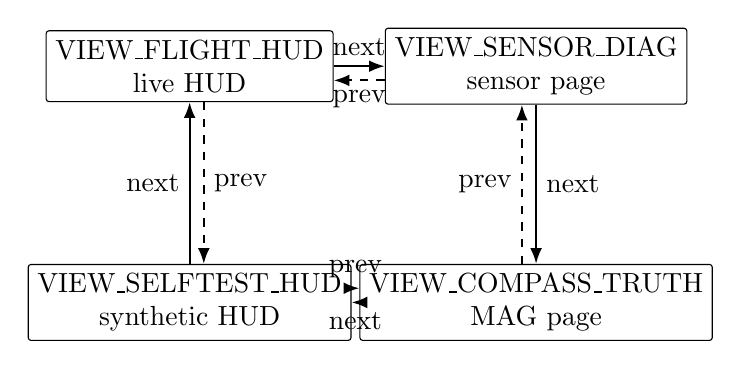
\begin{tikzpicture}[
  state/.style={draw, rounded corners=1pt, minimum width=3.0cm, minimum height=0.9cm, align=center},
  arr/.style={-{Latex[length=2mm]}, thick},
  rev/.style={-{Latex[length=2mm]}, thick, dashed}
]
\node[state] at (0,1.8) (hud) {\sig{VIEW\_FLIGHT\_HUD}\\live HUD};
\node[state] at (4.4,1.8) (diag) {\sig{VIEW\_SENSOR\_DIAG}\\sensor page};
\node[state] at (4.4,-1.2) (truth) {\sig{VIEW\_COMPASS\_TRUTH}\\MAG page};
\node[state] at (0,-1.2) (self) {\sig{VIEW\_SELFTEST\_HUD}\\synthetic HUD};

\draw[arr] (hud.east) -- node[above]{next} (diag.west);
\draw[arr] (diag.south) -- node[right]{next} (truth.north);
\draw[arr] (truth.west) -- node[below]{next} (self.east);
\draw[arr] (self.north) -- node[left]{next} (hud.south);

\draw[rev] ([yshift=-0.18cm]diag.west) -- node[below]{prev} ([yshift=-0.18cm]hud.east);
\draw[rev] ([xshift=-0.18cm]truth.north) -- node[left]{prev} ([xshift=-0.18cm]diag.south);
\draw[rev] ([yshift=0.18cm]self.east) -- node[above]{prev} ([yshift=0.18cm]truth.west);
\draw[rev] ([xshift=0.18cm]hud.south) -- node[right]{prev} ([xshift=0.18cm]self.north);
\end{tikzpicture}}
\caption{Phase 6 registered render-view state transitions.}
\end{figure}

\subsection{Legacy Hold Precedence}

For bench compatibility, the Phase 6 wrapper retains level-style legacy holds.
The effective view is not always the registered selected view:

\begin{center}
\begin{tabular}{l l}
\toprule
\textbf{Condition} & \textbf{\sig{view_effective_sys}} \\
\midrule
\sig{legacy_compass_page_hold_sys = 1} & \sig{VIEW_COMPASS_TRUTH} \\
\sig{legacy_selftest_hold_sys = 1} and compass hold is low & \sig{VIEW_SELFTEST_HUD} \\
otherwise & \sig{view_sel_sys} \\
\bottomrule
\end{tabular}
\end{center}

The precedence is deliberate: a held full-screen diagnostic page masks the HUD,
and the self-test HUD should only be visible when the compass page is not
forcing a full-screen replacement.

\subsection{Control-to-Renderer Mapping}

Figure~\ref{fig:control-renderer-map} maps the active top-level control path to
the renderer wrapper.  The control boundary produces independent self-test and
compass-page enables before final VGA compositing.

\begin{figure}[h]
\centering
\resizebox{\linewidth}{!}{%
\begin{tikzpicture}[
  box/.style={draw, rounded corners=1pt, text width=2.55cm, minimum height=0.78cm, align=center},
  wide/.style={draw, rounded corners=1pt, text width=3.15cm, minimum height=0.84cm, align=center},
  label/.style={align=center},
  arr/.style={-{Latex[length=2mm]}, thick},
  ctrl/.style={-{Latex[length=2mm]}, thick, dashed}
]
\node[label] at (0,3.25) {Active board-top wiring};
\node[box]  at (0,2.35) (cbtn) {BTNU/BTND/BTNR\\SW2/SW4/SW14};
\node[wide] at (3.15,2.35) (csplit) {sync/debounce\\view controls};
\node[wide] at (6.75,2.35) (csuite) {\file{caelumfusion_vga_render_control}\\view state};
\node[wide] at (10.35,2.35) (cpage) {HUD + optional\\compass page};
\node[box]  at (13.65,2.35) (cvga) {VGA pins\\HS, VS, RGB};
\node[box]  at (0,1.15) (csw) {\sig{sw_arm_raw}\\\sig{sw_policy_enable_raw}};
\node[wide] at (3.15,1.15) (cauth) {authority gate\\policy evidence};

\draw[arr]  (cbtn) -- (csplit);
\draw[ctrl] (csplit) -- (csuite);
\draw[arr]  (csuite) -- (cpage);
\draw[arr]  (cpage) -- (cvga);
\draw[arr]  (csw) -- (cauth);
\draw[arr]  (cauth) -| (csuite);

\draw[dashed] (-1.35,0.32) -- (14.85,0.32);

\node[label] at (0,-0.35) {Wrapper-internal selection};
\node[box]  at (0,-1.25) (pctl) {registered view\\legacy holds};
\node[wide] at (3.15,-1.25) (pwrap) {\file{caelumfusion_vga_render_control}\\legal view state};
\node[wide] at (6.75,-1.25) (pouts) {separate enables\\self-test, page};
\node[wide] at (10.35,-1.25) (prender) {same HUD + page\\renderer blocks};
\node[box]  at (13.65,-1.25) (pvga) {VGA pins\\HS, VS, RGB};

\draw[arr]  (pctl) -- (pwrap);
\draw[ctrl] (pwrap) -- (pouts);
\draw[ctrl] (pouts) -- (prender);
\draw[arr]  (prender) -- (pvga);
\end{tikzpicture}}
\caption{Control-to-renderer mapping.  Solid arrows carry telemetry or video;
dashed arrows carry control enables.}
\label{fig:control-renderer-map}
\end{figure}

\section{Configuration Map}

\subsection{Board Top Parameters}

\begin{longtable}{p{0.27\linewidth} p{0.15\linewidth} p{0.50\linewidth}}
\toprule
\textbf{Parameter} & \textbf{Default} & \textbf{Engineering meaning} \\
\midrule
\endhead
\param{SYS_CLK_HZ} & \sig{100_000_000} &
SYS-domain clock rate used by sensor jobs, timebase logic, and diagnostic page
update division. \\
\param{H_ACTIVE} & \sig{640} &
Active horizontal VGA pixels. \\
\param{H_FP} & \sig{16} &
Horizontal front porch. \\
\param{H_SYNC} & \sig{96} &
Horizontal sync pulse width. \\
\param{H_BP} & \sig{48} &
Horizontal back porch. \\
\param{V_ACTIVE} & \sig{480} &
Active vertical VGA lines. \\
\param{V_FP} & \sig{10} &
Vertical front porch. \\
\param{V_SYNC} & \sig{2} &
Vertical sync pulse height. \\
\param{V_BP} & \sig{33} &
Vertical back porch. \\
\param{HSYNC_POL} & \sig{0} &
0 means active-low hsync; 1 means active-high hsync. \\
\param{VSYNC_POL} & \sig{0} &
0 means active-low vsync; 1 means active-high vsync. \\
\param{BUILD_ID} & \sig{16'd4} &
Build metadata packed into the visualization bundle. \\
\param{ADXL_IRQ_POLICY} & \sig{1} &
Accelerometer interrupt sampling policy used by the sensor suite. \\
\param{USE_LIS3DH_I2C_ACC} & \sig{1} &
Default accelerometer source is the LIS3DH on shared I2C. \\
\param{USE_ADXL362_SPI_ACC} & \sig{0} &
ADXL362 SPI path is compiled out by default; when enabled by parameter
override, it can be selected by the runtime sensor-control switch. \\
\param{USE_CMPS2_MMC3416_MAG} & \sig{1} &
CMPS2/MMC34160PJ magnetometer heading path is enabled by default. \\
\param{USE_PMON1_PWR} & \sig{1} &
PMON1/ADM1191 power publication logic is present by source default and is gated
by the runtime PMON switch. \\
\param{PMON1_ADDR7} & \sig{7'h38} &
Configured PMON1 I2C address. \\
\param{USE_BLACKBOX_LOG} & \sig{0} &
Raw log packer is compiled out by default; when enabled by parameter override,
it is runtime-gated by SW6. \\
\param{USE_MAG1_BENCH_SOURCE} & \sig{0} &
Synthetic MAG1 bench source is compiled out by default; compile it in only for
bench-evidence builds, where it remains runtime-gated by SW3 and tagged as
synthetic. \\
\param{USE_COMPASS_TRUTH_PAGE} & \sig{0} &
Full-screen compass/MAG evidence page is compiled out by default for a smaller
HUD-only image.  Set this to nonzero for the BTNR/SW4/SW14 compass-page build. \\
\param{USE_SENSOR_DIAG_PAGE} & \sig{0} &
Sensor-diagnostic page RGB is compiled out by default.  The registered
\sig{VIEW_SENSOR_DIAG} state remains legal, but the PIX page mux emits the HUD
unless this parameter is nonzero. \\
\param{USE_SWITCH_ENCODED_VIEW_SELECT} & current RTL default nonzero &
When nonzero, BTNR direct selection samples SW13:SW11 only outside SW3 MAG1
bench and SW2+SW6 diagnostic fault-injection ownership.  Ownership collisions
force reserved \sig{3'b111} and preserve the registered view. \\
\param{COMPASS_TRUTH_PAGE_DEFAULT} & \sig{0} &
When the truth page is synthesized, this controls whether it boots as the
default visible page. \\
\bottomrule
\end{longtable}

\subsection{Phase 6 Wrapper Parameters}

\begin{longtable}{p{0.30\linewidth} p{0.17\linewidth} p{0.45\linewidth}}
\toprule
\textbf{Parameter} & \textbf{Active binding} & \textbf{Meaning} \\
\midrule
\endhead
\param{HIST_DEPTH} & \sig{1024} &
Depth of altitude and vertical-speed history rings in the visualization suite. \\
\param{MAG_PLOT_SHIFT} & \sig{8} &
Right-shift scaling applied to magnetic axes for compass truth-page plotting. \\
\param{ENABLE_SENSOR_DIAG_PAGE} & \sig{USE_SENSOR_DIAG_PAGE=0} &
Controls whether \sig{VIEW_SENSOR_DIAG} produces the diagnostic page RGB or
falls back to the primary HUD. \\
\param{ENABLE_COMPASS_TRUTH_PAGE} & \sig{USE_COMPASS_TRUTH_PAGE=0} &
Controls whether \sig{VIEW_COMPASS_TRUTH} is legal and whether the downstream
truth-page replacement stage is instantiated. \\
\param{RESET_VIEW_ID} & \sig{3'd0} &
Requested reset view.  Illegal reset values are coerced to
\sig{VIEW_FLIGHT_HUD}; if \param{COMPASS_TRUTH_PAGE_DEFAULT} is nonzero, reset
view becomes \sig{VIEW_COMPASS_TRUTH}. \\
\param{COMPASS_TRUTH_PAGE_DEFAULT} & \sig{0} &
Wrapper-owned boot-view policy.  The child truth page is instantiated with its
own default forced to 0 so it cannot permanently override the HUD. \\
\bottomrule
\end{longtable}

\subsection{Widget Enable and Degradation Controls}

The normal HUD does not use a large set of widget enable bits.  The engineering
contract is stronger: the screen geometry remains stable, and unavailable or
stale evidence is represented through color, hatch, marker suppression, or
empty history rather than by moving panels around.

\begin{longtable}{p{0.24\linewidth} p{0.24\linewidth} p{0.42\linewidth}}
\toprule
\textbf{Widget or layer} & \textbf{Enable/control source} & \textbf{Fallback or degradation behavior} \\
\midrule
\endhead
Top BMP/ACC/MAG health strip &
Always active in normal HUD during active video.  Uses raw
\sig{*_valid}, \sig{*_status}, \sig{*_age_ms}. &
Gray for unavailable, red for invalid/fault, yellow for stale or nonzero
warning status, green for valid/fresh/\sig{ST_OK}. \\

Telemetry text overlay &
Always available in normal HUD.  Text appears only where the compositor glyph
hit logic is true and active video is true. &
Text is clipped to top, panel, and bottom bands; no text pixel is emitted
outside the fixed clip windows. \\

Altitude tape and altitude chart &
Derived altitude plus BMP provenance:
\sig{der_valid}, \sig{der_alt_fresh}, \sig{der_bmp_valid_ref}. &
The panel remains drawn.  Color drops to gray/red/yellow when derived altitude
or BMP provenance is unavailable, faulty, or stale. \\

Vertical-speed tape and chart &
Derived vertical speed plus BMP provenance:
\sig{der_valid}, \sig{der_vspd_fresh}, \sig{der_bmp_valid_ref}. &
Positive and negative rates use different good colors; invalid or stale data
uses the same derived-state degradation policy as altitude. \\

Apogee authority ladder &
\sig{auth_valid}, \sig{auth_status}, target/prediction fields, command byte,
phase code, and gate flags. &
Unreachable or denied actuation changes envelope, command, phase, and gate
colors.  Invalid authority data hatches/de-emphasizes the panel rather than
removing it. \\

Artificial horizon and roll-plane vector &
\sig{der_roll_mdeg}, \sig{der_roll_fresh}, and ACC provenance. &
The reference geometry remains visible.  Roll quality hatch and semantic color
indicate stale or invalid attitude evidence. \\

Compass rose &
\sig{der_heading_mdeg}, \sig{der_head_fresh}, and MAG provenance. &
Heading needle quality degrades by color/hatching when MAG or derived heading
is invalid, stale, or not sequence-aligned. \\

Landing/wind viewport &
\sig{nav_valid}, \sig{nav_status}, \sig{nav_flags}, \sig{wind_valid},
\sig{wind_status}, and wind vector fields. &
Panel frame remains visible.  Navigation point and wind vector are suppressed
or warning-colored when upstream evidence is not valid. \\

Bottom debug strip &
Always active in normal HUD.  Uses PMON1 voltage/current/alert/age/sequence and
I2C NACK/timeout counters. &
Gray when PMON1 is intentionally unavailable, red for invalid/alert conditions,
yellow for stale or nonzero I2C error counters, white for clean power/debug
state. \\

Sensor diagnostic page &
Build-time \param{USE_SENSOR_DIAG_PAGE}; runtime
\sig{VIEW_SENSOR_DIAG} through \sig{vga_page_select_sys=2'd1}. &
If not synthesized, selecting \sig{VIEW_SENSOR_DIAG} leaves final HUD-stream RGB
on the primary HUD.  If synthesized, the diagnostic page replaces the primary
HUD page before the compass-truth overlay stage. \\

Compass truth page &
Build-time \param{USE_COMPASS_TRUTH_PAGE}; runtime \sig{page_enable_sys} or
Phase 6 \sig{compass_page_enable_sys}; optional
\param{COMPASS_TRUTH_PAGE_DEFAULT}. &
If not synthesized, final VGA is the normal HUD.  If synthesized but inactive,
sync and RGB pass through.  If active, RGB is replaced by page RGB while sync
passes through. \\
\bottomrule
\end{longtable}

\section{Semantic Visualization Bundle}

\subsection{Bundle Width and Regions}

The canonical visualization bundle is 1152 bits wide.  The map is intentionally
monotonic: legacy fields occupy the lower range, and newer evidence domains grow
upward.

\begin{center}
\begin{tabular}{r r l}
\toprule
\textbf{MSB} & \textbf{LSB} & \textbf{Region} \\
\midrule
1151 & 880 & Future sensor-extension evidence and black-box logging summary \\
879  & 800 & PMON1 / ADM1191 power-monitor evidence \\
799  & 640 & Navigation and wind estimator evidence \\
639  & 480 & Apogee authority / drag-servo policy evidence \\
479  & 357 & Raw BMP, ACC, MAG summaries \\
356  & 245 & Derived validity, freshness, provenance, and source references \\
244  & 117 & Derived altitude, vertical speed, roll, and heading numerics \\
116  & 1   & Platform counters, CDC count, build ID, and schema nibble \\
0    & 0   & Reserved \\
\bottomrule
\end{tabular}
\end{center}

\subsection{Publication Semantics}

The SYS-domain model emits a new semantic key when relevant source evidence
changes.  \file{flight_viz_suite_top} publishes a snapshot when the model key
changes, or when self-test mode produces a periodic liveness tick.  The
published bundle then crosses into the pixel domain.

The design intentionally separates three events:

\begin{enumerate}
  \item \textbf{SYS publication:} a coherent semantic image is captured in the
        SYS domain.
  \item \textbf{PIX CDC arrival:} the image becomes available as a PIX-domain
        shadow bundle.
  \item \textbf{Visible commit:} the renderer copies the shadow bundle into the
        committed visible bundle on \sig{vsync_edge}.
\end{enumerate}

This separation prevents mid-frame semantic tearing.  A new flight state can
arrive during active video, but it is not allowed to partially rewrite the
visible HUD until the next frame boundary.

\section{CDC and Frame-Stability Contract}

\subsection{SYS-to-PIX Snapshot CDC}

The bundle CDC is a low-rate snapshot transfer:

\begin{enumerate}
  \item \sig{src_publish_pulse} latches \sig{src_bundle} into
        \sig{src_bundle_hold}.
  \item The source domain toggles \sig{src_toggle}.
  \item The destination domain samples the toggle through a three-flop
        synchronizer.
  \item A detected toggle change captures \sig{src_bundle_hold} into
        \sig{dst_bundle_shadow}.
  \item \sig{dst_update_pulse} marks one PIX clock of new-shadow availability.
\end{enumerate}

This is not a bitwise synchronizer.  It is a snapshot CDC, and its correctness
depends on the source hold register remaining stable until the next publication.
That assumption is valid for the current low-rate telemetry and frame-rendering
use case.

\subsection{Frame-Boundary Commit}

The PIX renderer has two levels of bundle state:

\begin{itemize}
  \item \sig{viz_bundle_pix} and \sig{viz_update_pix}: incoming CDC shadow.
  \item \sig{viz_q}: committed visible bundle used for actual rendering.
\end{itemize}

When a CDC update arrives, the renderer stores it as pending.  On
\sig{vsync_edge}, the pending bundle becomes \sig{viz_q}.  The same pattern is
used for the chart write pointer, so chart cursors and semantic labels move
together at a frame boundary.

\section{Screen Layout Map}

\subsection{Raster Bands}

The active region is 640 by 480.  The current renderer uses fixed coordinate
bands:

\begin{center}
\begin{tabular}{r r l}
\toprule
\textbf{Y start} & \textbf{Y end} & \textbf{Function} \\
\midrule
0   & 27  & Compact top health strip for BMP, ACC, MAG \\
28  & 105 & Panel titles and text rows \\
106 & 359 & Primary instruments and authority/navigation panels \\
360 & 467 & Altitude and vertical-speed strip charts \\
468 & 479 & Bottom engineering/debug strip \\
\bottomrule
\end{tabular}
\end{center}

\subsection{Column Map}

\begin{center}
\begin{tabular}{r r l}
\toprule
\textbf{X start} & \textbf{X end} & \textbf{Primary content} \\
\midrule
0   & 212 & Altitude tape, vertical-speed tape, apogee authority envelope \\
213 & 425 & Artificial horizon and roll-plane vertical-vector instrument \\
426 & 639 & Compass rose, heading health, landing/wind viewport \\
\bottomrule
\end{tabular}
\end{center}

\subsection{Screen Layout Arrangement}

Figure~\ref{fig:screen-layout} shows the fixed normal-HUD arrangement in active
VGA coordinates.  The origin is the upper-left active pixel, with \(x\)
increasing to the right and \(y\) increasing downward.

\begin{figure}[h]
\centering
\resizebox{0.94\linewidth}{!}{%
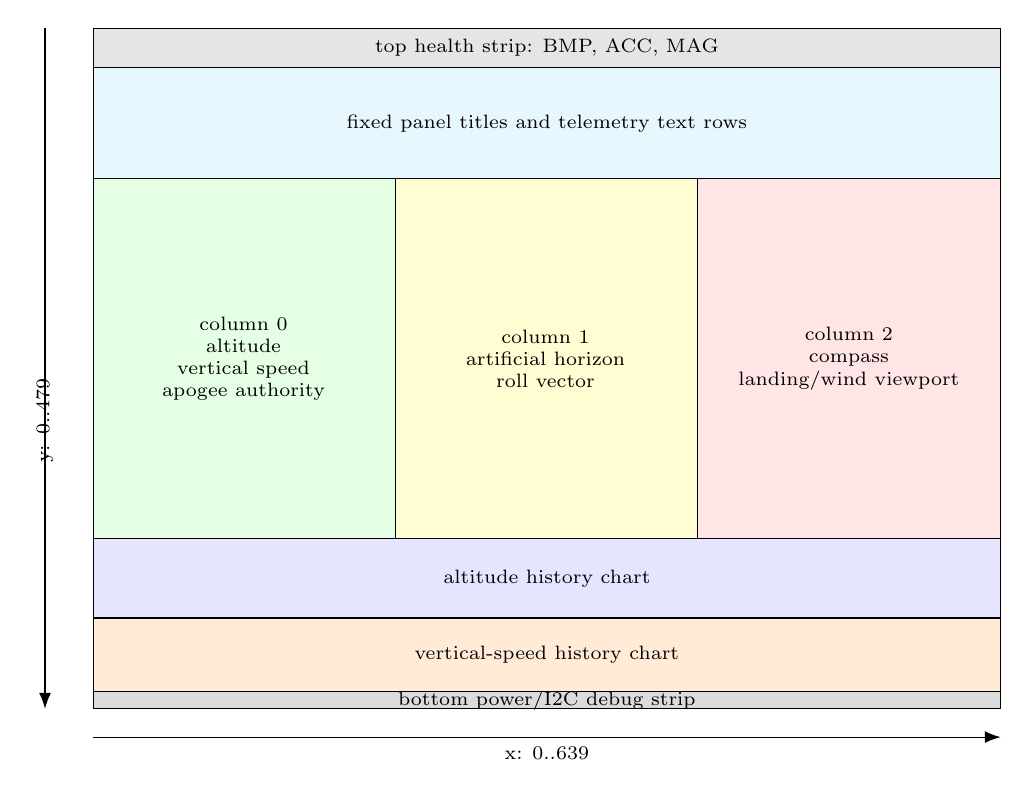
\begin{tikzpicture}[x=0.018cm,y=-0.018cm,font=\scriptsize]
  \draw[fill=black!4, draw=black] (0,0) rectangle (640,480);

  \draw[fill=gray!20, draw=black] (0,0) rectangle (640,28);
  \node at (320,14) {top health strip: BMP, ACC, MAG};

  \draw[fill=cyan!10, draw=black] (0,28) rectangle (640,106);
  \node at (320,67) {fixed panel titles and telemetry text rows};

  \draw[fill=green!10, draw=black] (0,106) rectangle (213,360);
  \node[align=center] at (106,233) {column 0\\altitude\\vertical speed\\apogee authority};

  \draw[fill=yellow!18, draw=black] (213,106) rectangle (426,360);
  \node[align=center] at (319,233) {column 1\\artificial horizon\\roll vector};

  \draw[fill=red!10, draw=black] (426,106) rectangle (640,360);
  \node[align=center] at (533,233) {column 2\\compass\\landing/wind viewport};

  \draw[fill=blue!10, draw=black] (0,360) rectangle (640,416);
  \node at (320,388) {altitude history chart};

  \draw[fill=orange!16, draw=black] (0,416) rectangle (640,468);
  \node at (320,442) {vertical-speed history chart};

  \draw[fill=gray!28, draw=black] (0,468) rectangle (640,480);
  \node at (320,474) {bottom power/I2C debug strip};

  \draw[-{Latex[length=2mm]}] (0,500) -- node[below]{x: 0..639} (640,500);
  \draw[-{Latex[length=2mm]}] (-34,0) -- node[left, rotate=90]{y: 0..479} (-34,480);
\end{tikzpicture}}
\caption{Normal HUD screen layout and viewport ownership.}
\label{fig:screen-layout}
\end{figure}

\subsection{Sensor Diagnostic Page Arrangement}

When \param{USE_SENSOR_DIAG_PAGE != 0} and
\sig{VIEW_SENSOR_DIAG} is selected, \file{flight_visualizer_pix.v} replaces the
primary HUD page RGB inside the HUD-stream page mux.  The normal telemetry text
compositor is intentionally suppressed for this page.  The diagnostic layout is
fixed:

\begin{center}
\begin{tabular}{l r r l}
\toprule
\textbf{Diagnostic region} & \textbf{X range} & \textbf{Y range} & \textbf{Visible evidence} \\
\midrule
Sensor matrix & 8--314 & 36--284 &
BMP, ACC, MAG, PWR, derived, extension, navigation, and wind rows. \\
Extension scales & 330--628 & 36--222 &
Range, airspeed, temperature, humidity, sun, and optical-flow scale bars. \\
Navigation/wind trail & 330--628 & 246--452 &
Current and recent navigation/wind points with invalid-evidence hatching. \\
\bottomrule
\end{tabular}
\end{center}

\begin{figure}[h]
\centering
\resizebox{0.94\linewidth}{!}{%
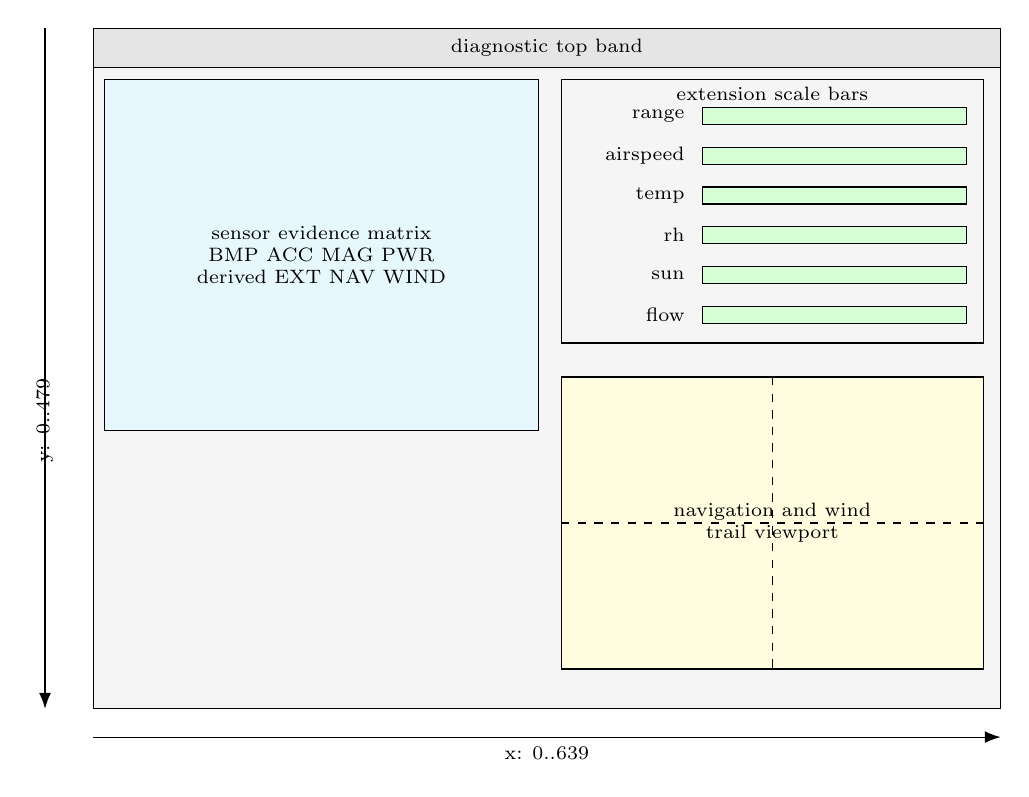
\begin{tikzpicture}[x=0.018cm,y=-0.018cm,font=\scriptsize]
  \draw[fill=black!4, draw=black] (0,0) rectangle (640,480);

  \draw[fill=gray!20, draw=black] (0,0) rectangle (640,28);
  \node at (320,14) {diagnostic top band};

  \draw[fill=cyan!10, draw=black] (8,36) rectangle (314,284);
  \node[align=center] at (161,160) {sensor evidence matrix\\BMP ACC MAG PWR\\derived EXT NAV WIND};

  \foreach \yy/\name in {56/range,84/airspeed,112/temp,140/rh,168/sun,196/flow} {
    \draw[fill=green!16, draw=black] (430,\yy) rectangle (616,\yy+12);
    \node[anchor=east] at (424,\yy+6) {\name};
  }
  \draw[draw=black] (330,36) rectangle (628,222);
  \node at (479,46) {extension scale bars};

  \draw[fill=yellow!12, draw=black] (330,246) rectangle (628,452);
  \draw[dashed] (479,246) -- (479,452);
  \draw[dashed] (330,349) -- (628,349);
  \node[align=center] at (479,349) {navigation and wind\\trail viewport};

  \draw[-{Latex[length=2mm]}] (0,500) -- node[below]{x: 0..639} (640,500);
  \draw[-{Latex[length=2mm]}] (-34,0) -- node[left, rotate=90]{y: 0..479} (-34,480);
\end{tikzpicture}}
\caption{Sensor diagnostic page screen arrangement.}
\label{fig:sensor-diag-layout}
\end{figure}

\subsection{Text Overlay Geometry}

Text is rendered through a shared 3-by-5 glyph datapath.  The compositor uses
fixed-width ASCII buses and fixed clipping bands so text cannot spill into
instrument centers.

\begin{longtable}{p{0.22\linewidth} p{0.18\linewidth} p{0.16\linewidth} p{0.34\linewidth}}
\toprule
\textbf{Region} & \textbf{Origin(s)} & \textbf{Width} & \textbf{Contract} \\
\midrule
\endhead
Top health strip &
\sig{(20,6)}, \sig{(226,6)}, \sig{(432,6)} &
15 chars each &
BMP, ACC, and MAG validity/status/age/sequence fields. \\

Panel titles &
\sig{(10,30)}, \sig{(236,30)}, \sig{(456,30)} &
18 chars each &
Permanent labels: \sig{ALT VSPD AUTH}, \sig{HORIZON ATT}, and
\sig{HEADING HEALTH}. \\

Panel telemetry rows &
\sig{Y=44,56,68,80,92} &
18 chars each &
Roll/provenance, altitude/vertical speed, and heading/provenance summaries. \\

Bottom debug strip &
\sig{(10,470)} &
48 chars &
Power-monitor, alert, sequence, NACK, and timeout evidence using 1x glyphs. \\
\bottomrule
\end{longtable}

\section{Color Conventions}

\subsection{RGB444 Palette Usage}

The VGA output is RGB444.  The renderer frequently builds colors as
\sig{\{R[3:0],G[3:0],B[3:0]\}}, while the text generator assigns RGB888-style
semantic colors that are truncated to RGB444 by the final overlay stage.  The
table below documents the visible meaning rather than every literal color
constant.

\begin{longtable}{p{0.20\linewidth} p{0.22\linewidth} p{0.48\linewidth}}
\toprule
\textbf{Color family} & \textbf{Representative RGB444 codes} & \textbf{Engineering meaning} \\
\midrule
\endhead
Black &
\sig{12'h000} &
Inactive video, reset/blanking, or empty background.  The final HUD mux forces
black whenever active video is false. \\

Dim grid / frame &
\sig{12'h011}, \sig{12'h022}, \sig{12'h044}, \sig{12'h111} &
Low-salience coordinate grids, panel frames, and inactive instrument context. \\

White &
\sig{12'hFFF}, \sig{12'hCCC}, \sig{12'hAAA} &
Primary labels, center dots, reference axes, current markers, and clean status
text where no semantic warning color is required. \\

Cyan / blue &
\sig{12'h0FF}, \sig{12'h3FF}, \sig{12'h08F} &
Heading text, vector accents, redundant MAG1/reference plotting, and
instrument accents. \\

Green &
\sig{12'h0F4}, \sig{12'h2F6}, \sig{12'h2B5} &
Valid, fresh, reachable, aligned, or allowed state.  Green is reserved for
positive evidence, not merely for decorative emphasis. \\

Yellow / amber &
\sig{12'hFF0}, \sig{12'hFD0}, \sig{12'hD93} &
Stale evidence, warning status, freshness miss, sequence mismatch, or caution
state that is still representable. \\

Orange &
\sig{12'hF80}, \sig{12'hF50}, \sig{12'hF42} &
Commanded/braking/boost-style emphasis, warning fill, or degraded but active
diagnostic vector. \\

Red &
\sig{12'hF22}, \sig{12'hF50}, \sig{12'hD33} &
Invalid, faulted, denied, disagreeing, or unsafe evidence. \\

Magenta &
\sig{12'hF0F} &
MAG live-vector accent and brake-phase emphasis. \\
\bottomrule
\end{longtable}

\subsection{Semantic Color Rules}

\begin{longtable}{p{0.22\linewidth} p{0.27\linewidth} p{0.41\linewidth}}
\toprule
\textbf{Evidence class} & \textbf{Inputs inspected} & \textbf{Color rule} \\
\midrule
\endhead
Raw BMP/ACC/MAG text &
\sig{valid}, \sig{status}, \sig{age_ms}, stale threshold &
Gray when unavailable, red when invalid, yellow when status is nonzero or age is
past threshold, green when valid/fresh/\sig{ST_OK}. \\

Derived left/right text &
\sig{der_valid}, \sig{der_status}, per-axis freshness &
Gray when the derived subsystem is unavailable, red for invalid, yellow for
nonzero status or stale axis, green when valid and fresh. \\

Derived middle text &
\sig{der_valid}, \sig{der_status}, \sig{der_alt_fresh},
\sig{der_vspd_fresh} &
Requires both altitude and vertical speed freshness for green.  Either stale
axis downgrades the middle panel to yellow. \\

Authority panel &
\sig{auth_valid}, \sig{auth_status}, reachability, command level, phase code,
gate flags &
Reachable/allows-actuation cases use green or cyan accents.  Denied, unsafe,
or unreachable cases use orange/red.  Missing authority evidence is gray. \\

Bottom debug strip &
\sig{pwr_valid}, \sig{pwr_status}, \sig{pwr_age_ms}, \sig{pwr_alert},
\sig{i2c_nack_count}, \sig{i2c_timeout_count} &
White for clean PMON1/I2C state, gray for intentionally unavailable PMON1,
yellow for stale or single-counter warning, red for invalid power status,
alerts, or both I2C error counters active. \\

Compass truth page &
MAG validity/status/age, derived heading freshness, sequence match, redundant
MAG agreement, extension fault flags &
Green for good heading evidence, yellow for stale/mismatch/warning, red for
invalid/fault/disagreement, blue/cyan/magenta for primary versus redundant
vector identity. \\
\bottomrule
\end{longtable}

\section{Render Layer Priority}

\subsection{Normal Flight HUD}

The normal HUD renderer uses \file{flight_vga_page_mux_pix} as its final
PIX-domain page selector.  It has three final output rules:

\begin{enumerate}
  \item If active video is false, RGB is forced to black.
  \item Else if the selected page is the primary HUD and text overlay is active,
        text RGB overrides the primary HUD scene.
  \item Else the selected page RGB is emitted.  The selected page is either the
        primary HUD scene or the sensor-diagnostic page.
\end{enumerate}

In RTL form:

\begin{lstlisting}
assign vga_rgb =
    (!active_pix) ? 12'h000 :
    (telemetry_overlay_on && !sensor_diag_page) ? telemetry_overlay_rgb :
                                                  page_rgb;
\end{lstlisting}

This priority is the correct engineering behavior: inactive video must be
black; labels and numeric evidence must remain readable on the primary HUD; and
the sensor-diagnostic page remains unobscured when it is selected.

\subsection{Compass Truth Page Overlay}

The optional truth page is a stream replacement stage after the normal HUD:

\begin{lstlisting}
assign vga_hsync_out = vga_hsync_in;
assign vga_vsync_out = vga_vsync_in;
assign vga_rgb_out   = page_active ? page_rgb_r : vga_rgb_in;
\end{lstlisting}

The page does not generate a new board-facing sync contract.  It passes the
existing VGA sync through and replaces active RGB when selected.  This matters
because the truth page is an overlay on the VGA stream, not a separate display
interface.

\subsection{Compositor Layer Stack}

Figure~\ref{fig:layer-stack} shows the final RGB priority from lowest to
highest.  The normal HUD base scene and optional sensor diagnostic page are
formed inside \file{flight_visualizer_pix}.  The page mux then selects one of
those page RGB sources, applies HUD-only text overlay, forces inactive-video
black, and finally the optional compass truth page can replace the already
formed HUD-stream RGB when selected.

\begin{figure}[h]
\centering
\resizebox{0.92\linewidth}{!}{%
\begin{tikzpicture}[
  layer/.style={draw, rounded corners=1pt, minimum width=11.4cm, minimum height=0.72cm, align=center},
  note/.style={draw, rounded corners=1pt, text width=5.25cm, align=center},
  arr/.style={-{Latex[length=2mm]}, thick}
]
\node[layer, fill=gray!10] at (0,0) (grid) {lowest: background grid, panel frames, base instrument geometry};
\node[layer, fill=green!10] at (0,0.90) (base) {primary HUD markers: tapes, authority, horizon, compass, landing/wind, charts};
\node[layer, fill=blue!10] at (0,1.80) (diag) {sensor-diagnostic page RGB when selected and compiled in};
\node[layer, fill=cyan!10] at (0,2.70) (text) {HUD-only text overlay: top health, panel rows, bottom debug};
\node[layer, fill=black!10] at (0,3.60) (blank) {HUD-stream final mux: inactive video forces \sig{12'h000}};
\node[layer, fill=orange!14] at (0,4.50) (page) {optional truth-page RGB replacement when \sig{page_active=1}};
\draw[arr] (-6.2,0) -- node[left, rotate=90]{priority increases} (-6.2,4.5);
\node[note] at (-2.95,-1.05) {Inside each page, later conditional assignments intentionally override lower-salience grid pixels.};
\node[note] at (2.95,-1.05) {The truth page replaces RGB only.  It passes \sig{vga_hsync} and \sig{vga_vsync} through unchanged.};
\end{tikzpicture}}
\caption{Compositor layer stack and final VGA routing priority.}
\label{fig:layer-stack}
\end{figure}

\section{Diagnostic Views}

\subsection{Flight HUD}

The flight HUD is the default display.  It renders:

\begin{itemize}
  \item raw BMP, ACC, and MAG validity/status/age/sequence health;
  \item derived altitude, vertical speed, roll, and heading;
  \item source-provenance links from derived state back to raw sequences;
  \item apogee authority target, predicted no-brake/full-brake apogee, command
        evidence, uncertainty, phase, and gate status;
  \item artificial horizon and roll-plane vertical-vector instrument;
  \item compass rose and heading quality;
  \item landing dispersion / wind estimator viewport when valid evidence is
        available;
  \item bottom power and I2C diagnostic strip.
\end{itemize}

\subsection{Self-Test HUD}

Self-test HUD mode is not a separate renderer.  It is the normal HUD fed by
deterministic synthetic evidence inside \file{flight_viz_suite_top}.  The mode
is useful for proving display activity, layout, colors, history rings, and text
without live sensors.  It must be treated as representation-test evidence, not
flight truth.

\subsection{Sensor Diagnostic Page}

The sensor diagnostic page is a secondary page inside the normal HUD renderer.
It is selected by \sig{VIEW_SENSOR_DIAG} through
\sig{vga_page_select_sys=2'd1}.  The page is compiled only when
\param{USE_SENSOR_DIAG_PAGE != 0}; otherwise the same selected view falls back
to primary HUD RGB.  When present, the diagnostic page displays:

\begin{itemize}
  \item a left-side sensor evidence matrix for BMP, ACC, MAG, PWR, derived,
        extension, navigation, and wind validity/status/age/fault state;
  \item upper-right extension scale bars for range, airspeed, temperature,
        relative humidity, sun/luma, and optical-flow magnitude;
  \item lower-right navigation/wind trail history with current-point markers
        and hatching when evidence is invalid or stale.
\end{itemize}

The page is deliberately graphical and status-oriented.  It does not render the
normal telemetry text overlay, and it should be used as a bring-up and
integration diagnostic rather than as a flight-facing primary HUD.

\subsection{Planar Compass Truth Page}

The compass truth page is a full-screen diagnostic for the CMPS2/MMC34160PJ
heading path.  It displays:

\begin{itemize}
  \item sensor identity and address context;
  \item planar heading from raw magnetic axes;
  \item MAG status, age, freshness, and sequence;
  \item raw MX/MY live vector and 16-sample trail;
  \item approximate magnetic field norm gauge;
  \item FPGA heading versus raw-sector crosscheck;
  \item I2C NACK, timeout, and transaction-rate evidence.
\end{itemize}

The heading is explicitly a planar \(\operatorname{atan2}(M_Y,M_X)\) style
diagnostic.  It is not a tilt-compensated navigation heading unless the upstream
derived-state pipeline has explicitly added and documented tilt compensation.

\section{Telemetry Fields Shown in Each Mode}

\subsection{Normal Flight HUD and Self-Test HUD}

\sig{VIEW_FLIGHT_HUD} and \sig{VIEW_SELFTEST_HUD} use the same visible HUD
geometry.  The difference is the source of the fields: live telemetry in flight
HUD mode, deterministic \sig{SELFTEST_*} substitutions in self-test HUD mode.

\begin{longtable}{p{0.20\linewidth} p{0.32\linewidth} p{0.38\linewidth}}
\toprule
\textbf{VGA region} & \textbf{Visible text or graphical field} & \textbf{Source contract} \\
\midrule
\endhead
Top health strip &
\sig{BMP V ST AGE SQ}, \sig{ACC V ST AGE SQ}, \sig{MAG V ST AGE SQ} where
\sig{V} is valid/missing, \sig{ST} is status hex, \sig{AGE} is decimal age, and
\sig{SQ} is sequence low byte. &
Raw BMP/ACC/MAG \sig{valid}, \sig{status}, \sig{age_ms}, and \sig{seq}. \\

Left panel text &
\sig{ROLL +/-dddd deg}, \sig{RFRS}, \sig{ACCV}, \sig{AAGE}, \sig{ASEQ},
\sig{ATT DERIVED ACC}. &
Derived roll angle, roll freshness, ACC valid reference, ACC reference age, and
ACC sequence reference. \\

Middle panel text &
\sig{ALT +/-dddddd cm}, \sig{VSPD +/-dddddd cm/s}, \sig{AF}, \sig{VF},
\sig{DV}, \sig{BREF}, \sig{BSEQ}, \sig{ST}. &
Derived altitude, vertical speed, altitude freshness, vertical-speed freshness,
derived-valid bit, BMP reference validity/age/sequence, and derived status. \\

Right panel text &
\sig{HEAD ddddd deg}, \sig{HFRS}, \sig{MAGV}, \sig{MAGE}, \sig{MSEQ},
\sig{HDG DERIVED MAG}. &
Derived heading, heading freshness, MAG reference validity, MAG reference age,
and MAG sequence reference. \\

Bottom debug strip &
\sig{PV}, \sig{PI}, \sig{AL}, \sig{AG}, \sig{SQ}, \sig{NK}, \sig{TO}. &
PMON1 voltage code, current code, alert status, power age, power sequence,
I2C NACK count, and I2C timeout count. \\

Graphical instruments &
Altitude tape, vertical-speed tape, apogee ladder, artificial horizon,
roll-plane vector, compass rose, landing/wind viewport, altitude chart, and
vertical-speed chart. &
Derived state, authority evidence, raw/derived provenance, navigation/wind
evidence, and BRAM-backed history samples. \\

Carried but not currently printed &
\sig{cdc_update_count}, \sig{build_id}, \sig{schema_word}, full raw payloads,
and several extension fields. &
These fields are packed into the visualization bundle and available for later
debug-page expansion, but the current bottom strip does not render them. \\
\bottomrule
\end{longtable}

\subsection{Sensor Diagnostic Page}

\sig{VIEW_SENSOR_DIAG} uses the same committed visualization bundle as the
primary HUD, but displays it through diagnostic matrices and scale bars instead
of the normal text overlay.  The page has no additional telemetry transport
contract beyond the bundle already delivered to \file{flight_visualizer_pix.v}.

\begin{longtable}{p{0.22\linewidth} p{0.31\linewidth} p{0.37\linewidth}}
\toprule
\textbf{Page region} & \textbf{Visible field} & \textbf{Source contract} \\
\midrule
\endhead
Sensor evidence matrix &
Eight fixed rows for BMP, ACC, MAG, PWR, derived state, extension group,
navigation, and wind.  Each row encodes validity, status, age/freshness, and
fault state through colored row cells and an age bar. &
Committed bundle fields including \sig{*_valid}, \sig{*_status},
\sig{*_age_ms}, derived freshness flags, extension fault flags, and PMON alert. \\

Extension scale bars &
Range, airspeed, temperature, relative humidity, sun/luma, and optical-flow
magnitude bars. &
\sig{ext_rng_height_cm}, \sig{ext_air_speed_cms}, \sig{ext_env_temp_cdeg},
\sig{ext_env_rh_centi}, \sig{ext_sun_luma}, \sig{ext_flow_dx},
\sig{ext_flow_dy}, plus extension presence and stale/fault flags. \\

Navigation/wind trail &
Current navigation point, current wind point, and 16-sample recent trail for
each when valid.  Invalid or stale evidence produces a warning hatch in the
trail viewport. &
\sig{nav_valid}, \sig{nav_status}, \sig{nav_downrange_m},
\sig{nav_crossrange_m}, \sig{wind_valid}, \sig{wind_status},
\sig{wind_x_cms}, and \sig{wind_y_cms}. \\
\bottomrule
\end{longtable}

\subsection{Compass Truth Page}

The compass truth page is a focused diagnostic view for the MAG/heading path.
It is intentionally more raw than the normal HUD: it exposes primary and
redundant magnetic evidence, sequence alignment, disagreement flags, and I2C
error counters.

\begin{longtable}{p{0.22\linewidth} p{0.31\linewidth} p{0.37\linewidth}}
\toprule
\textbf{Page region} & \textbf{Visible field} & \textbf{Source contract} \\
\midrule
\endhead
Header and page labels &
Page title, planar-compass wording, sensor/source labels, and warning that the
heading is planar. &
Static diagnostic labels generated in the truth-page renderer. \\

Left compass rose &
Heading in degrees, compass needle, good/warn/fault color state, and heading
age/status/sequence. &
\sig{der_heading_mdeg}, \sig{der_head_fresh}, \sig{mag_valid},
\sig{mag_status}, \sig{mag_age_ms}, and \sig{mag_seq}. \\

Center MX/MY plot &
Live primary MAG vector, 16-sample primary trail, optional redundant MAG1
vector, and plot axes. &
\sig{mag_payload[47:0]} and \sig{mag1_payload[47:0]} using
\sig{\{MZ,MY,MX\}} packing and \param{MAG_PLOT_SHIFT} scaling. \\

Right status badge &
Good/warning/fault badge, MAG age, MAG sequence, MAG status, heading freshness,
and derived-to-raw sequence crosscheck. &
Primary MAG and derived heading freshness/provenance fields. \\

Redundant MAG evidence panel &
Presence flags, extension status, fault flags, primary/secondary norm metrics,
L1 delta, max age, disagreement, pair-missing, and norm-fault conditions. &
\sig{ext_valid}, \sig{ext_status}, \sig{ext_present_flags},
\sig{ext_fault_flags}, \sig{ext_mag_delta_l1}, \sig{ext_mag_norm_primary},
\sig{ext_mag_norm_secondary}, and \sig{ext_max_age_ms}. \\

Bottom-left raw axes and norm gauges &
Primary \sig{MX}, \sig{MY}, \sig{MZ}, approximate norm, redundant delta and norm
bars. &
Primary MAG payload, redundant MAG payload, extension delta/norm fields, and
derived health state. \\

Bottom-right crosscheck and I2C diagnostics &
FPGA heading, published/raw sector comparison, \sig{OK}/\sig{BAD} crosscheck,
I2C NACK count, timeout count, and transaction rate. &
\sig{der_heading_mdeg}, raw sector from \sig{MX/MY}, \sig{i2c_nack_count},
\sig{i2c_timeout_count}, and \sig{txn_rate_hz}. \\

MAG1 detail column &
\sig{M1X}, \sig{M1Y}, \sig{M1Z}, valid/status, sequence/age, alignment,
sector delta, disagreement, norm delta, iron residual, calibration state,
source flags, and bridge checksum. &
\sig{mag1_*} and redundant-MAG extension bridge fields. \\
\bottomrule
\end{longtable}

\section{Truth, Representation, and Evidence Boundaries}

The VGA renderer is an engineering instrument, so this document uses the
following evidence categories:

\begin{center}
\begin{tabularx}{\linewidth}{p{0.22\linewidth} X}
\toprule
\textbf{Category} & \textbf{Meaning} \\
\midrule
Raw evidence &
Sensor publication fields such as sequence, valid, status, payload, and age.
These are nearest to the sensor transaction layer. \\

Derived evidence &
Computed altitude, vertical speed, roll, heading, freshness flags, and sequence
references.  These are estimates and must preserve provenance. \\

Authority evidence &
Apogee policy status, target, predictions, brake command, servo pulse, phase,
and gate bits.  This is flight-control decision evidence, not just graphics. \\

Display representation &
Pixels, colors, glyphs, plotted vectors, and chart points derived from the
evidence.  Representation can be clipped, saturated, or symbolically encoded. \\

Diagnostic self-test &
Synthetic evidence used to validate rendering behavior.  It must not be
mistaken for live flight telemetry. \\

Sensor diagnostic page &
HUD-stream diagnostic representation of sensor validity, extension health, and
navigation/wind trails.  It is selected before normal HUD text overlay and does
not change the committed telemetry bundle. \\

Compass truth page &
Focused diagnostic representation of the magnetometer/heading pipeline.  It
can replace the visible HUD but does not change the underlying sensor contract. \\
\bottomrule
\end{tabularx}
\end{center}

\section{Verification Map}

\subsection{Existing Simulation Evidence}

The source tree already includes self-checking tests that cover substantial
parts of the VGA path.

\begin{longtable}{p{0.32\linewidth} p{0.58\linewidth}}
\toprule
\textbf{Testbench} & \textbf{Relevant checks} \\
\midrule
\endhead
\file{tb_flight_visualizer_pix.v} &
Checks active/inactive video behavior, 24-bit to 12-bit text color packing,
overlay priority, clipping, chart newest-sample markers, attitude instruments,
apogee authority markers, denied-gate indication, bottom debug strip, and black
inactive output. \\

\file{tb_flight_viz_suite_top.v} &
Checks SYS semantic publication, CDC delivery into PIX shadow bundle, history
ring storage, known text pixel output, and landing/wind viewport response. \\

\file{caelumfusion_top_vga_i2c_tb.v} &
Checks top-level clock/reset, I2C activity, sensor snapshot resolution, VGA sync
activity, and nonzero known RGB output in a behavioral top-level simulation. \\
\bottomrule
\end{longtable}

\subsection{Phase 6 Additions Required}

Before claiming Phase 6 render-control closure, add or extend tests for:

\begin{enumerate}
  \item Reset selects a legal \sig{view_sel_sys} for every legal and illegal
        \param{RESET_VIEW_ID} value.
  \item \sig{view_next_pulse_sys} and \sig{view_prev_pulse_sys} cycle through
        \sig{VIEW_FLIGHT_HUD}, \sig{VIEW_SENSOR_DIAG},
        \sig{VIEW_COMPASS_TRUTH}, and \sig{VIEW_SELFTEST_HUD} when the compass
        page is enabled.
  \item With \param{USE_COMPASS_TRUTH_PAGE=0}, next/previous skip
        \sig{VIEW_COMPASS_TRUTH} and direct compass requests or encoded ID
        \sig{3'd1} latch \sig{cfg_invalid_view_sys}.
  \item With encoded direct selection active, SW3 MAG1 bench mode and SW2+SW6
        fault injection force BTNR requests to reserved \sig{3'b111}; the
        selected view must hold and \sig{cfg_invalid_view_sys} must latch.
  \item With \param{USE_SENSOR_DIAG_PAGE=0}, \sig{VIEW_SENSOR_DIAG} remains
        selectable but the visible HUD-stream RGB falls back to the primary HUD.
  \item With \param{USE_SENSOR_DIAG_PAGE=1}, \sig{VIEW_SENSOR_DIAG} selects the
        sensor evidence matrix, extension scale bars, and navigation/wind trail,
        and the normal telemetry text overlay is suppressed.
  \item Illegal direct view IDs do not change \sig{view_sel_sys} and do latch
        \sig{cfg_invalid_view_sys}.
  \item \sig{cfg_invalid_view_clear_sys} clears only the invalid-view latch and
        does not change the selected view.
  \item \sig{legacy_compass_page_hold_sys} overrides both registered view and
        self-test hold.
  \item \sig{legacy_selftest_hold_sys} overrides the registered view only when
        compass page hold is low.
  \item In self-test HUD mode, the compass truth page remains inactive.
  \item In compass truth-page mode, the normal HUD still generates timing and
        sync, but final RGB is replaced by page RGB.
  \item View-control pulses are already synchronized and debounced before they
        enter the wrapper; asynchronous button sampling is tested separately.
\end{enumerate}

\subsection{Implementation and Bench Gates}

The release checklist should be updated with the following VGA-specific Phase 6
gates:

\begin{itemize}
  \item Vivado elaboration confirms one active board top and no accidental
        duplicate renderer source copies in the active source set.
  \item Routed timing remains clean for both SYS and generated PIX clocks.
  \item CDC exceptions remain scoped to reviewed snapshot buses and toggle
        synchronizers only.
  \item Default build with \param{USE_COMPASS_TRUTH_PAGE=0} and
        \param{USE_SENSOR_DIAG_PAGE=0} still meets LUT margin expectations.
  \item Optional builds with \param{USE_COMPASS_TRUTH_PAGE=1} and/or
        \param{USE_SENSOR_DIAG_PAGE=1} record utilization delta, timing slack,
        and DRC deltas.
  \item Bench video confirms stable VGA sync, active display, correct reset
        default view, and no mid-frame tearing during view changes.
  \item Bench sensor perturbations show validity, freshness, stale, and error
        conditions visibly distinct on VGA.
\end{itemize}

\section{Default and Fallback Display Behavior}

\begin{longtable}{p{0.26\linewidth} p{0.32\linewidth} p{0.32\linewidth}}
\toprule
\textbf{Condition} & \textbf{Default behavior} & \textbf{Reasoning} \\
\midrule
\endhead
Power-on or reset &
Timing outputs return to registered idle values and RGB remains black until the
pixel clock/reset path is released and a committed bundle is available. &
Avoids random colored pixels during reset and keeps sync behavior deterministic. \\

Default board parameters &
\param{USE_COMPASS_TRUTH_PAGE=0}, \param{USE_SENSOR_DIAG_PAGE=0}, and
\param{COMPASS_TRUTH_PAGE_DEFAULT=0}. &
The source-default build boots to the normal flight HUD and keeps optional page
logic out of the image unless a page-enabled build overrides the parameters. \\

Compass page not synthesized &
Direct or held compass-page requests are rejected or gated by
\param{ENABLE_COMPASS_TRUTH_PAGE=0}. &
Final VGA is assigned directly from the HUD stream; self-test remains available
through the explicit self-test hold. \\

Sensor diagnostic page not synthesized &
\sig{VIEW_SENSOR_DIAG} remains a legal registered view, but
\file{flight_visualizer_pix.v} forces \sig{render_page_select_q} back to the
HUD page when \param{ENABLE_SENSOR_DIAG_PAGE=0}. &
Navigation can still exercise the registered view state without introducing a
blank or undefined diagnostic page. \\

Compass page synthesized but not selected &
Truth-page module passes \sig{vga_hsync}, \sig{vga_vsync}, and
\sig{vga_rgb} through from the HUD stream. &
Diagnostic overlay is additive and does not own a separate sync generator at
the final board interface. \\

Inactive video or blanking &
RGB is forced to \sig{12'h000}. &
Prevents semantic pixels from appearing during blanking intervals. \\

Invalid raw sensor evidence &
Panel geometry remains fixed; health and derived colors degrade to gray, red,
or yellow. &
The display remains an engineering instrument instead of hiding missing data. \\

Navigation or wind evidence invalid &
\sig{nav_valid=0}, \sig{wind_valid=0}, nonzero status, stale age, or invalid
freshness suppresses or warning-colors the landing/wind viewport and sensor
diagnostic trail. &
The renderer visibly degrades rather than implying a valid zero crossrange or
zero wind solution. \\

Illegal Phase 6 direct view ID &
The wrapper holds the current selected view and latches
\sig{cfg_invalid_view_sys}. &
Reserved encodings cannot decode into arbitrary video routing. \\

Invalid-view latch in the current board top &
\sig{cfg_invalid_view_clear_sys} is tied to \sig{1'b0} in
\file{caelumfusion_top_vga.v}. &
The latch is clearable inside the wrapper interface, but the board-level image
currently clears it only by reset. \\

Illegal Phase 6 reset view &
\param{RESET_VIEW_ID} is coerced to \sig{VIEW_FLIGHT_HUD}, unless
\param{COMPASS_TRUTH_PAGE_DEFAULT} requests \sig{VIEW_COMPASS_TRUTH}. &
Reset is deterministic even when a parameter is misconfigured. \\
\bottomrule
\end{longtable}

\section{Known Rendering Limitations}

\begin{longtable}{p{0.25\linewidth} p{0.35\linewidth} p{0.30\linewidth}}
\toprule
\textbf{Limitation} & \textbf{Current state} & \textbf{Impact} \\
\midrule
\endhead
Render-control status visibility &
\sig{view_sel_sys}, \sig{view_effective_sys}, and \sig{cfg_invalid_view_sys}
are internal top-level wires. &
The board can select views, but invalid-view/debug status is not yet exposed on
LEDs, UART, or a persisted telemetry field. \\

Feature-rich build resource cost &
Optional page and peripheral builds can enable the compass page, sensor
diagnostic page, MAG1 bench source, ADXL362 path, and black-box log packer. &
Synthesis/implementation must be re-run after each feature change to confirm LUT
margin and timing on the Artix-7 35T. \\

Fixed debounce interval &
View buttons use \sig{STABLE_CYCLES=250000} in the SYS clock domain. &
This is deterministic but not runtime tunable; very fast repeated button taps
inside the debounce window are intentionally ignored. \\

25.000 MHz VGA pixel clock &
The design uses 25.000 MHz rather than the nominal 25.175 MHz 640x480 VGA
clock. &
The frame rate is about 59.524 Hz.  Most monitors accept this, but strict
timing documentation should record the approximation. \\

RGB444 analog output &
The Basys-3 VGA path exposes four bits per channel through the board resistor
DAC. &
Color gradients, anti-aliased text, and fine diagnostic shading are intentionally
coarse. \\

Fixed 3-by-5 glyphs &
Text uses a compact glyph map with 2x scaling for normal text and 1x for the
bottom debug strip. &
Labels are deterministic and cheap, but not typographically rich; long fields
must be abbreviated. \\

Fixed layout &
Normal HUD widget positions are compile-time constants. &
There is no runtime layout manager, zoom mode, or pan/scroll behavior. \\

No top-level data-enable pin &
The board output exposes sync and RGB only; active video is internal to the VGA
renderer. &
A future digital encoder should derive an explicit \sig{VGA_de} from the same
active-video timing contract. \\
\bottomrule
\end{longtable}

\section{Known Risks and Open Items}

\begin{longtable}{p{0.20\linewidth} p{0.42\linewidth} p{0.28\linewidth}}
\toprule
\textbf{Risk} & \textbf{Current condition} & \textbf{Recommended resolution} \\
\midrule
\endhead
Implementation closure &
The wrapper integration elaborates, but the latest batch synthesis attempt did
not reach \sig{synth_design} in the Codex run environment. &
Re-run synthesis and implementation from Vivado and record utilization, WNS/WHS,
DRC, and bitstream evidence for the default HUD build and optional page-enabled
builds. \\

Control observability &
View state and invalid-view latch are not currently routed to a visible debug
field. &
Expose \sig{view_effective_sys} and \sig{cfg_invalid_view_sys} on a small HUD
debug field or LED/UART hook for bench validation. \\

Stale terminology &
Some historical comments in the source tree may still mention HDMI as a future
or mistaken display label. &
Remove or reword those comments so all display documentation says VGA unless a
real digital-video encoder is added. \\

Legacy artifact reconciliation &
Older report artifacts used HDMI-oriented or pre-wrapper terminology. &
Treat this document and the active RTL as the source-aligned control map; if a
legacy artifact is retained, mark it superseded or revise its terminology. \\
\bottomrule
\end{longtable}

\section{Recommended Phase 6 Development Sequence}

\begin{enumerate}
  \item \textbf{Add a render-control testbench.}  Exercise next/previous/direct
        selection, disabled-compass rejection, legacy hold priority, and the
        invalid-view latch.
  \item \textbf{Expose view diagnostics.}  Route \sig{view_effective_sys} and
        \sig{cfg_invalid_view_sys} to a small debug field, LEDs, or UART-visible
        status so bench testing can distinguish selected, held, and rejected
        views.
  \item \textbf{Run focused simulation.}  Re-run the pixel renderer, suite top,
        render-control wrapper, and board-level VGA activity tests.
  \item \textbf{Run implementation deltas.}  Record utilization, WNS, WHS, DRC,
        and bitstream hash for the source-default HUD build, a
        \param{USE_COMPASS_TRUTH_PAGE=1} build, and a
        \param{USE_SENSOR_DIAG_PAGE=1} build.
  \item \textbf{Capture bench evidence.}  Photograph or record VGA output for
        reset default, live telemetry, stale/error conditions, self-test HUD,
        and compass truth page.
\end{enumerate}

\section{Traceability Summary}

\begin{center}
\begin{tabularx}{\linewidth}{p{0.26\linewidth} X}
\toprule
\textbf{Requirement} & \textbf{Trace path} \\
\midrule
VGA-only output &
\file{Basys-3-Master.xdc} maps only \sig{vga_hsync}, \sig{vga_vsync}, and
\sig{vga_rgb[11:0]} display pins; no HDMI/TMDS ports are present. \\

Frame-stable HUD &
\file{flight_visualizer_pix.v} commits \sig{viz_q} and chart pointer state on
\sig{vsync_edge}. \\

Semantic CDC &
\file{flight_viz_bundle_cdc.v} and scoped XDC false paths define a held-bundle
toggle CDC between SYS and PIX. \\

Observable health &
\file{flight_viz_telemetry_textgen.v} and \file{flight_visualizer_pix.v}
preserve validity, status, age, freshness, sequence, and platform counters in
visible text/colors. \\

Diagnostic page isolation &
\file{planar_compass_truth_page_vga.v} replaces RGB only when active and passes
sync through unchanged. \\

Phase 6 view separation &
\file{caelumfusion_vga_render_control.v} defines separate legal views and
separate \sig{flight_selftest_en_sys} / \sig{compass_page_enable_sys} outputs. \\
Sensor diagnostic isolation &
\file{flight_vga_page_mux_pix.v} selects the sensor diagnostic page before
normal HUD text overlay and suppresses text overlay for the diagnostic page. \\
\bottomrule
\end{tabularx}
\end{center}

\section{Conclusion}

The corrected Phase 6 display contract is VGA-only.  The active Basys-3 design
drives \sig{vga_hsync}, \sig{vga_vsync}, and \sig{vga_rgb[11:0]} from a
25.000 MHz pixel-domain renderer with 640 by 480 active timing.  The rendering
pipeline is already structured around coherent SYS-domain semantic publication,
explicit SYS-to-PIX snapshot CDC, frame-boundary visible commits, and an active
\file{caelumfusion_vga_render_control.v} wrapper.  The main remaining Phase 6
work is verification and observability: add focused render-control tests,
expose selected/invalid view state on a bench-visible channel, and refresh
synthesis/implementation evidence for the default and page-enabled builds.

\end{document}
